\documentclass[twoside]{book}

% Packages required by doxygen
\usepackage{fixltx2e}
\usepackage{calc}
\usepackage{doxygen}
\usepackage[export]{adjustbox} % also loads graphicx
\usepackage{graphicx}
\usepackage[utf8]{inputenc}
\usepackage{makeidx}
\usepackage{multicol}
\usepackage{multirow}
\PassOptionsToPackage{warn}{textcomp}
\usepackage{textcomp}
\usepackage[nointegrals]{wasysym}
\usepackage[table]{xcolor}

% Font selection
\usepackage[T1]{fontenc}
\usepackage[scaled=.90]{helvet}
\usepackage{courier}
\usepackage{amssymb}
\usepackage{sectsty}
\renewcommand{\familydefault}{\sfdefault}
\allsectionsfont{%
  \fontseries{bc}\selectfont%
  \color{darkgray}%
}
\renewcommand{\DoxyLabelFont}{%
  \fontseries{bc}\selectfont%
  \color{darkgray}%
}
\newcommand{\+}{\discretionary{\mbox{\scriptsize$\hookleftarrow$}}{}{}}

% Page & text layout
\usepackage{geometry}
\geometry{%
  a4paper,%
  top=2.5cm,%
  bottom=2.5cm,%
  left=2.5cm,%
  right=2.5cm%
}
\tolerance=750
\hfuzz=15pt
\hbadness=750
\setlength{\emergencystretch}{15pt}
\setlength{\parindent}{0cm}
\setlength{\parskip}{3ex plus 2ex minus 2ex}
\makeatletter
\renewcommand{\paragraph}{%
  \@startsection{paragraph}{4}{0ex}{-1.0ex}{1.0ex}{%
    \normalfont\normalsize\bfseries\SS@parafont%
  }%
}
\renewcommand{\subparagraph}{%
  \@startsection{subparagraph}{5}{0ex}{-1.0ex}{1.0ex}{%
    \normalfont\normalsize\bfseries\SS@subparafont%
  }%
}
\makeatother

% Headers & footers
\usepackage{fancyhdr}
\pagestyle{fancyplain}
\fancyhead[LE]{\fancyplain{}{\bfseries\thepage}}
\fancyhead[CE]{\fancyplain{}{}}
\fancyhead[RE]{\fancyplain{}{\bfseries\leftmark}}
\fancyhead[LO]{\fancyplain{}{\bfseries\rightmark}}
\fancyhead[CO]{\fancyplain{}{}}
\fancyhead[RO]{\fancyplain{}{\bfseries\thepage}}
\fancyfoot[LE]{\fancyplain{}{}}
\fancyfoot[CE]{\fancyplain{}{}}
\fancyfoot[RE]{\fancyplain{}{\bfseries\scriptsize Generated by Doxygen }}
\fancyfoot[LO]{\fancyplain{}{\bfseries\scriptsize Generated by Doxygen }}
\fancyfoot[CO]{\fancyplain{}{}}
\fancyfoot[RO]{\fancyplain{}{}}
\renewcommand{\footrulewidth}{0.4pt}
\renewcommand{\chaptermark}[1]{%
  \markboth{#1}{}%
}
\renewcommand{\sectionmark}[1]{%
  \markright{\thesection\ #1}%
}

% Indices & bibliography
\usepackage{natbib}
\usepackage[titles]{tocloft}
\setcounter{tocdepth}{3}
\setcounter{secnumdepth}{5}
\makeindex

% Hyperlinks (required, but should be loaded last)
\usepackage{ifpdf}
\ifpdf
  \usepackage[pdftex,pagebackref=true]{hyperref}
\else
  \usepackage[ps2pdf,pagebackref=true]{hyperref}
\fi
\hypersetup{%
  colorlinks=true,%
  linkcolor=blue,%
  citecolor=blue,%
  unicode%
}

% Custom commands
\newcommand{\clearemptydoublepage}{%
  \newpage{\pagestyle{empty}\cleardoublepage}%
}

\usepackage{caption}
\captionsetup{labelsep=space,justification=centering,font={bf},singlelinecheck=off,skip=4pt,position=top}

%===== C O N T E N T S =====

\begin{document}

% Titlepage & ToC
\hypersetup{pageanchor=false,
             bookmarksnumbered=true,
             pdfencoding=unicode
            }
\pagenumbering{alph}
\begin{titlepage}
\vspace*{7cm}
\begin{center}%
{\Large R\+W\+A2\+\_\+\+Group\+\_\+1\+\_\+1 \\[1ex]\large 0.\+1 }\\
\vspace*{1cm}
{\large Generated by Doxygen 1.8.13}\\
\end{center}
\end{titlepage}
\clearemptydoublepage
\pagenumbering{roman}
\tableofcontents
\clearemptydoublepage
\pagenumbering{arabic}
\hypersetup{pageanchor=true}

%--- Begin generated contents ---
\chapter{Maze search algorithm}
\label{index}\hypertarget{index}{}This project consists of searching a path in a maze and then task a mouse (robot) to follow the path.
\begin{DoxyItemize}
\item \hyperlink{searchingPathPage}{Searching a path}
\item \hyperlink{followingPathPage}{Following a path} 
\end{DoxyItemize}
\chapter{Searching a path}
\label{searching_path_page}
\Hypertarget{searching_path_page}
The search algorithm used for searching a path in a maze relies on the depth-\/first search (D\+FS) approach. This algorithm is implemented in \hyperlink{classrwa2_1_1_mouse_a66b3d6d831d814a569401158b07f9e83}{rwa2\+::\+Mouse\+::search\+\_\+maze()} 
\chapter{Following a path}
\label{following_path_page}
\Hypertarget{following_path_page}
To follow a path generated by D\+FS, methods from the class A\+PI (api/api.\+h) must be used to interact with the micromouse simulator.
\begin{DoxyItemize}
\item Methods of the A\+PI class are documented \href{https://github.com/mackorone/mms#summary}{\tt here}. 
\end{DoxyItemize}
\chapter{Class Index}
\section{Class List}
Here are the classes, structs, unions and interfaces with brief descriptions\+:\begin{DoxyCompactList}
\item\contentsline{section}{\hyperlink{classrwa2_1_1_mouse}{rwa2\+::\+Mouse} \\*This class is used to compute a path and execute the path }{\pageref{classrwa2_1_1_mouse}}{}
\end{DoxyCompactList}

\chapter{File Index}
\section{File List}
Here is a list of all documented files with brief descriptions\+:\begin{DoxyCompactList}
\item\contentsline{section}{include/mouse/\hyperlink{mouse_8h}{mouse.\+h} \\*The file contains the Mouse class }{\pageref{mouse_8h}}{}
\end{DoxyCompactList}

\chapter{Class Documentation}
\hypertarget{classrwa2_1_1_mouse}{}\section{rwa2\+:\+:Mouse Class Reference}
\label{classrwa2_1_1_mouse}\index{rwa2\+::\+Mouse@{rwa2\+::\+Mouse}}


This class is used to compute a path and execute the path.  




{\ttfamily \#include $<$mouse.\+h$>$}

\subsection*{Public Member Functions}
\begin{DoxyCompactItemize}
\item 
\hyperlink{classrwa2_1_1_mouse_a048dffae3aaa3a6ddc2c6cc4741a097c}{Mouse} ()
\begin{DoxyCompactList}\small\item\em Construct a new Micro\+Mouse object. \end{DoxyCompactList}\item 
void \hyperlink{classrwa2_1_1_mouse_a6bbb329ddb93efbab9f7c91134cc1d44}{log} (const std\+::string \&text)
\begin{DoxyCompactList}\small\item\em Print string onto A\+PI. \end{DoxyCompactList}\item 
\mbox{\Hypertarget{classrwa2_1_1_mouse_abbcc99c41fd073426fdfd790f947956e}\label{classrwa2_1_1_mouse_abbcc99c41fd073426fdfd790f947956e}} 
void \hyperlink{classrwa2_1_1_mouse_abbcc99c41fd073426fdfd790f947956e}{display\+\_\+walls} ()
\begin{DoxyCompactList}\small\item\em Visually set the walls in the simulator. \end{DoxyCompactList}\item 
bool \hyperlink{classrwa2_1_1_mouse_a66b3d6d831d814a569401158b07f9e83}{search\+\_\+maze} (std\+::pair$<$ int, int $>$ \&n)
\begin{DoxyCompactList}\small\item\em Implement D\+FS to compute a path between current node and goal node in a maze. \end{DoxyCompactList}\item 
\mbox{\Hypertarget{classrwa2_1_1_mouse_afc6e0d56e3a777c05efa3929eb256e0a}\label{classrwa2_1_1_mouse_afc6e0d56e3a777c05efa3929eb256e0a}} 
void \hyperlink{classrwa2_1_1_mouse_afc6e0d56e3a777c05efa3929eb256e0a}{move\+\_\+forward} ()
\begin{DoxyCompactList}\small\item\em Make the mouse move forward. \end{DoxyCompactList}\item 
\mbox{\Hypertarget{classrwa2_1_1_mouse_a5748e94e740432c334d15364fb476919}\label{classrwa2_1_1_mouse_a5748e94e740432c334d15364fb476919}} 
void \hyperlink{classrwa2_1_1_mouse_a5748e94e740432c334d15364fb476919}{turn\+\_\+left} ()
\begin{DoxyCompactList}\small\item\em Make the mouse rotate 90 deg C\+CW. \end{DoxyCompactList}\item 
\mbox{\Hypertarget{classrwa2_1_1_mouse_ac929127d86fc4a41d1e216968b1dae20}\label{classrwa2_1_1_mouse_ac929127d86fc4a41d1e216968b1dae20}} 
void \hyperlink{classrwa2_1_1_mouse_ac929127d86fc4a41d1e216968b1dae20}{turn\+\_\+right} ()
\begin{DoxyCompactList}\small\item\em Make the mouse rotate 90 deg CW. \end{DoxyCompactList}\item 
\mbox{\Hypertarget{classrwa2_1_1_mouse_a7ca431550bf9f8b27f904b20f77519f4}\label{classrwa2_1_1_mouse_a7ca431550bf9f8b27f904b20f77519f4}} 
void \hyperlink{classrwa2_1_1_mouse_a7ca431550bf9f8b27f904b20f77519f4}{program\+\_\+flow} ()
\begin{DoxyCompactList}\small\item\em Implement Algorithm 2 to move mouse in the simulator. \end{DoxyCompactList}\item 
bool \hyperlink{classrwa2_1_1_mouse_a5de2232aada66b8fa3a640fcb0554761}{find} (const std\+::vector$<$ std\+::pair$<$ int, int $>$$>$ \&list, const std\+::pair$<$ int, int $>$ \&element)
\begin{DoxyCompactList}\small\item\em Search for an element in a list, stack or vector. \end{DoxyCompactList}\item 
bool \hyperlink{classrwa2_1_1_mouse_aba15def87bc971a1b4f02252ab53c600}{set\+\_\+maze\+\_\+walls} (const std\+::pair$<$ int, int $>$ \&path\+\_\+node)
\begin{DoxyCompactList}\small\item\em Draws wall on the simulation and stores wall information from the simulation to the maze program. \end{DoxyCompactList}\item 
void \hyperlink{classrwa2_1_1_mouse_a496eaae99071570dfa4b9328e1462ce7}{turn\+\_\+mouse} (const std\+::pair$<$ int, int $>$ \&nxt\+\_\+step)
\begin{DoxyCompactList}\small\item\em Turns the mouse to face the next tile it\textquotesingle{}s going to step on. \end{DoxyCompactList}\item 
\mbox{\Hypertarget{classrwa2_1_1_mouse_a00888982dc159f0ee01718e6b59104aa}\label{classrwa2_1_1_mouse_a00888982dc159f0ee01718e6b59104aa}} 
void \hyperlink{classrwa2_1_1_mouse_a00888982dc159f0ee01718e6b59104aa}{follow\+\_\+path} ()
\begin{DoxyCompactList}\small\item\em Take found path and move mouse. If wall is detected, re-\/search maze and set appropriate walls. \end{DoxyCompactList}\item 
void \hyperlink{classrwa2_1_1_mouse_a844c61c266db3edb980b9f6d30edaf6f}{reverse\+\_\+stack} (std\+::stack$<$ std\+::pair$<$ int, int $>$$>$ \&stack)
\begin{DoxyCompactList}\small\item\em Flip the order of (x,y) nodes in solution stack. \end{DoxyCompactList}\item 
\mbox{\Hypertarget{classrwa2_1_1_mouse_a1d9828afd97b16dc64d941af6504223d}\label{classrwa2_1_1_mouse_a1d9828afd97b16dc64d941af6504223d}} 
void \hyperlink{classrwa2_1_1_mouse_a1d9828afd97b16dc64d941af6504223d}{draw\+\_\+path} ()
\begin{DoxyCompactList}\small\item\em Draws color of the final path of the mouse on the simulation using reverse\+\_\+stack and color path functions. \end{DoxyCompactList}\item 
void \hyperlink{classrwa2_1_1_mouse_ac855fa63f17bb4ea650401ad2dae44b6}{color\+\_\+path} (const std\+::stack$<$ std\+::pair$<$ int, int $>$$>$ \&path)
\begin{DoxyCompactList}\small\item\em color found path in white and goal node in green \end{DoxyCompactList}\end{DoxyCompactItemize}


\subsection{Detailed Description}
This class is used to compute a path and execute the path. 

Definition at line 53 of file mouse.\+h.



\subsection{Constructor \& Destructor Documentation}
\mbox{\Hypertarget{classrwa2_1_1_mouse_a048dffae3aaa3a6ddc2c6cc4741a097c}\label{classrwa2_1_1_mouse_a048dffae3aaa3a6ddc2c6cc4741a097c}} 
\index{rwa2\+::\+Mouse@{rwa2\+::\+Mouse}!Mouse@{Mouse}}
\index{Mouse@{Mouse}!rwa2\+::\+Mouse@{rwa2\+::\+Mouse}}
\subsubsection{\texorpdfstring{Mouse()}{Mouse()}}
{\footnotesize\ttfamily rwa2\+::\+Mouse\+::\+Mouse (\begin{DoxyParamCaption}{ }\end{DoxyParamCaption})\hspace{0.3cm}{\ttfamily [inline]}}



Construct a new Micro\+Mouse object. 

The robot is always at (0,0) and facing N\+O\+R\+TH when the simulator starts The goal node is initialized in the mouse ctor The body of the ctor sets boundary walls in the internal maze 

Definition at line 63 of file mouse.\+h.



\subsection{Member Function Documentation}
\mbox{\Hypertarget{classrwa2_1_1_mouse_ac855fa63f17bb4ea650401ad2dae44b6}\label{classrwa2_1_1_mouse_ac855fa63f17bb4ea650401ad2dae44b6}} 
\index{rwa2\+::\+Mouse@{rwa2\+::\+Mouse}!color\+\_\+path@{color\+\_\+path}}
\index{color\+\_\+path@{color\+\_\+path}!rwa2\+::\+Mouse@{rwa2\+::\+Mouse}}
\subsubsection{\texorpdfstring{color\+\_\+path()}{color\_path()}}
{\footnotesize\ttfamily void rwa2\+::\+Mouse\+::color\+\_\+path (\begin{DoxyParamCaption}\item[{const std\+::stack$<$ std\+::pair$<$ int, int $>$$>$ \&}]{path }\end{DoxyParamCaption})}



color found path in white and goal node in green 


\begin{DoxyParams}{Parameters}
{\em path} & being inputted to color route accordingly \\
\hline
\end{DoxyParams}
\mbox{\Hypertarget{classrwa2_1_1_mouse_a5de2232aada66b8fa3a640fcb0554761}\label{classrwa2_1_1_mouse_a5de2232aada66b8fa3a640fcb0554761}} 
\index{rwa2\+::\+Mouse@{rwa2\+::\+Mouse}!find@{find}}
\index{find@{find}!rwa2\+::\+Mouse@{rwa2\+::\+Mouse}}
\subsubsection{\texorpdfstring{find()}{find()}}
{\footnotesize\ttfamily bool rwa2\+::\+Mouse\+::find (\begin{DoxyParamCaption}\item[{const std\+::vector$<$ std\+::pair$<$ int, int $>$$>$ \&}]{list,  }\item[{const std\+::pair$<$ int, int $>$ \&}]{element }\end{DoxyParamCaption})}



Search for an element in a list, stack or vector. 


\begin{DoxyParams}{Parameters}
{\em list} & the 1D stack or vector being searched \\
\hline
{\em element} & the variable, ordered pair in search\\
\hline
\end{DoxyParams}
\begin{DoxyReturn}{Returns}
true if that element exists 

false if the element does not exist 
\end{DoxyReturn}
\mbox{\Hypertarget{classrwa2_1_1_mouse_a6bbb329ddb93efbab9f7c91134cc1d44}\label{classrwa2_1_1_mouse_a6bbb329ddb93efbab9f7c91134cc1d44}} 
\index{rwa2\+::\+Mouse@{rwa2\+::\+Mouse}!log@{log}}
\index{log@{log}!rwa2\+::\+Mouse@{rwa2\+::\+Mouse}}
\subsubsection{\texorpdfstring{log()}{log()}}
{\footnotesize\ttfamily void rwa2\+::\+Mouse\+::log (\begin{DoxyParamCaption}\item[{const std\+::string \&}]{text }\end{DoxyParamCaption})}



Print string onto A\+PI. 


\begin{DoxyParams}{Parameters}
{\em text} & String being inputted to be displayed. \\
\hline
\end{DoxyParams}
\mbox{\Hypertarget{classrwa2_1_1_mouse_a844c61c266db3edb980b9f6d30edaf6f}\label{classrwa2_1_1_mouse_a844c61c266db3edb980b9f6d30edaf6f}} 
\index{rwa2\+::\+Mouse@{rwa2\+::\+Mouse}!reverse\+\_\+stack@{reverse\+\_\+stack}}
\index{reverse\+\_\+stack@{reverse\+\_\+stack}!rwa2\+::\+Mouse@{rwa2\+::\+Mouse}}
\subsubsection{\texorpdfstring{reverse\+\_\+stack()}{reverse\_stack()}}
{\footnotesize\ttfamily void rwa2\+::\+Mouse\+::reverse\+\_\+stack (\begin{DoxyParamCaption}\item[{std\+::stack$<$ std\+::pair$<$ int, int $>$$>$ \&}]{stack }\end{DoxyParamCaption})}



Flip the order of (x,y) nodes in solution stack. 


\begin{DoxyParams}{Parameters}
{\em stack} & \\
\hline
\end{DoxyParams}
\mbox{\Hypertarget{classrwa2_1_1_mouse_a66b3d6d831d814a569401158b07f9e83}\label{classrwa2_1_1_mouse_a66b3d6d831d814a569401158b07f9e83}} 
\index{rwa2\+::\+Mouse@{rwa2\+::\+Mouse}!search\+\_\+maze@{search\+\_\+maze}}
\index{search\+\_\+maze@{search\+\_\+maze}!rwa2\+::\+Mouse@{rwa2\+::\+Mouse}}
\subsubsection{\texorpdfstring{search\+\_\+maze()}{search\_maze()}}
{\footnotesize\ttfamily bool rwa2\+::\+Mouse\+::search\+\_\+maze (\begin{DoxyParamCaption}\item[{std\+::pair$<$ int, int $>$ \&}]{n }\end{DoxyParamCaption})}



Implement D\+FS to compute a path between current node and goal node in a maze. 


\begin{DoxyParams}{Parameters}
{\em n} & current node for search, an ordered pair (x, y)\\
\hline
\end{DoxyParams}
\begin{DoxyReturn}{Returns}
true A path is found 

false A path is not found 
\end{DoxyReturn}
\mbox{\Hypertarget{classrwa2_1_1_mouse_aba15def87bc971a1b4f02252ab53c600}\label{classrwa2_1_1_mouse_aba15def87bc971a1b4f02252ab53c600}} 
\index{rwa2\+::\+Mouse@{rwa2\+::\+Mouse}!set\+\_\+maze\+\_\+walls@{set\+\_\+maze\+\_\+walls}}
\index{set\+\_\+maze\+\_\+walls@{set\+\_\+maze\+\_\+walls}!rwa2\+::\+Mouse@{rwa2\+::\+Mouse}}
\subsubsection{\texorpdfstring{set\+\_\+maze\+\_\+walls()}{set\_maze\_walls()}}
{\footnotesize\ttfamily bool rwa2\+::\+Mouse\+::set\+\_\+maze\+\_\+walls (\begin{DoxyParamCaption}\item[{const std\+::pair$<$ int, int $>$ \&}]{path\+\_\+node }\end{DoxyParamCaption})}



Draws wall on the simulation and stores wall information from the simulation to the maze program. 


\begin{DoxyParams}{Parameters}
{\em path\+\_\+node} & an ordered pair holding values of current nodes \\
\hline
\end{DoxyParams}
\begin{DoxyReturn}{Returns}
true if the method finishes without mouse hitting a wall 

false if new wall exists 
\end{DoxyReturn}
\mbox{\Hypertarget{classrwa2_1_1_mouse_a496eaae99071570dfa4b9328e1462ce7}\label{classrwa2_1_1_mouse_a496eaae99071570dfa4b9328e1462ce7}} 
\index{rwa2\+::\+Mouse@{rwa2\+::\+Mouse}!turn\+\_\+mouse@{turn\+\_\+mouse}}
\index{turn\+\_\+mouse@{turn\+\_\+mouse}!rwa2\+::\+Mouse@{rwa2\+::\+Mouse}}
\subsubsection{\texorpdfstring{turn\+\_\+mouse()}{turn\_mouse()}}
{\footnotesize\ttfamily void rwa2\+::\+Mouse\+::turn\+\_\+mouse (\begin{DoxyParamCaption}\item[{const std\+::pair$<$ int, int $>$ \&}]{nxt\+\_\+step }\end{DoxyParamCaption})}



Turns the mouse to face the next tile it\textquotesingle{}s going to step on. 


\begin{DoxyParams}{Parameters}
{\em nxt\+\_\+step} & Ordered pair which is the difference of current node with the next node in the final path \\
\hline
\end{DoxyParams}


The documentation for this class was generated from the following file\+:\begin{DoxyCompactItemize}
\item 
include/mouse/\hyperlink{mouse_8h}{mouse.\+h}\end{DoxyCompactItemize}

\chapter{File Documentation}
\hypertarget{mouse_8h}{}\section{include/mouse/mouse.h File Reference}
\label{mouse_8h}\index{include/mouse/mouse.\+h@{include/mouse/mouse.\+h}}


The file contains the Mouse class.  


{\ttfamily \#include \char`\"{}../node/node.\+h\char`\"{}}\newline
{\ttfamily \#include \char`\"{}../util/util.\+h\char`\"{}}\newline
{\ttfamily \#include $<$stack$>$}\newline
{\ttfamily \#include $<$string$>$}\newline
{\ttfamily \#include $<$vector$>$}\newline
{\ttfamily \#include $<$utility$>$}\newline
Include dependency graph for mouse.\+h\+:\nopagebreak
\begin{figure}[H]
\begin{center}
\leavevmode
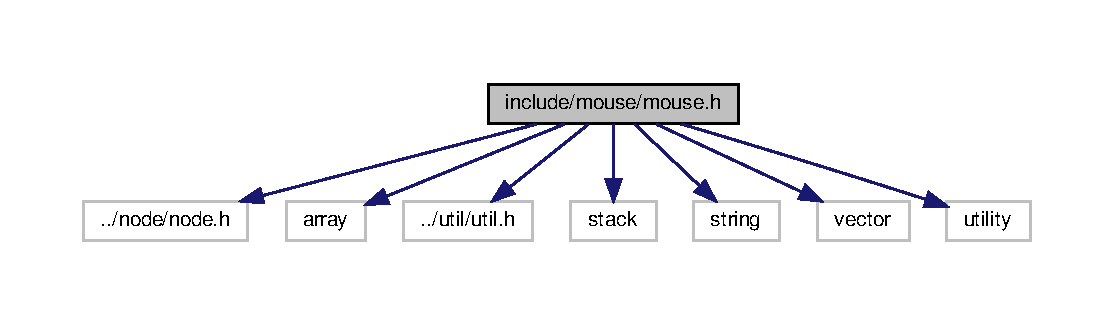
\includegraphics[width=350pt]{mouse_8h__incl}
\end{center}
\end{figure}
\subsection*{Classes}
\begin{DoxyCompactItemize}
\item 
class \hyperlink{classrwa2_1_1_mouse}{rwa2\+::\+Mouse}
\begin{DoxyCompactList}\small\item\em This class is used to compute a path and execute the path. \end{DoxyCompactList}\end{DoxyCompactItemize}


\subsection{Detailed Description}
The file contains the Mouse class. 

\begin{DoxyAuthor}{Author}
Hae Lee Kim, Yoseph Kebede, Mohammed Baaqeel 
\end{DoxyAuthor}
\begin{DoxyVersion}{Version}
0.\+1 
\end{DoxyVersion}
\begin{DoxyDate}{Date}
2021-\/11-\/12
\end{DoxyDate}
\begin{DoxyCopyright}{Copyright}
Copyright (c) 2021 
\end{DoxyCopyright}

%--- End generated contents ---

% Index
\backmatter
\newpage
\phantomsection
\clearemptydoublepage
\addcontentsline{toc}{chapter}{Index}
\printindex

\end{document}
